\let\negmedspace\undefined
\let\negthickspace\undefined
\documentclass[journal]{IEEEtran}
\usepackage[a5paper, margin=10mm, onecolumn]{geometry}
%\usepackage{lmodern} % Ensure lmodern is loaded for pdflatex
\usepackage{tfrupee} % Include tfrupee package

\setlength{\headheight}{1cm} % Set the height of the header box
\setlength{\headsep}{0mm}     % Set the distance between the header box and the top of the text

\usepackage{gvv-book}
\usepackage{hyperref}
\usepackage{gvv}
\usepackage{cite}
\usepackage{amsmath,amssymb,amsfonts,amsthm}
\usepackage{algorithmic}
\usepackage{graphicx}
\usepackage{textcomp}
\usepackage{xcolor}
\usepackage{txfonts}
\usepackage{listings}
\usepackage{enumitem}
\usepackage{mathtools}
\usepackage{gensymb}
\usepackage{comment}
\usepackage[breaklinks=true]{hyperref}
\usepackage{tkz-euclide} 
\usepackage{listings}
% \usepackage{gvv}                                        
\def\inputGnumericTable{}                                 
\usepackage[latin1]{inputenc}                                
\usepackage{color}                                            
\usepackage{array}                                            
\usepackage{longtable}                                       
\usepackage{calc}                                             
\usepackage{multirow}                                         
\usepackage{hhline}                                           
\usepackage{ifthen}                                           
\usepackage{lscape}
\usepackage{circuitikz}
\usepackage{titlesec}
\usepackage{placeins}
\usepackage{pgfplots}
\usepackage{booktabs}
\usepackage{setspace}
\usepackage{hyperref}
\usepackage{xcolor}
\usepackage{tikz}
\usepackage{listings}
\usepackage{xcolor}
\tikzstyle{block} = [rectangle, draw, fill=blue!20, 
    text width=4em, text centered, rounded corners, minimum height=3em]
\tikzstyle{sum} = [draw, fill=blue!10, circle, minimum size=1cm, node distance=1.5cm]
\tikzstyle{input} = [coordinate]
\tikzstyle{output} = [coordinate]
\titleformat{\section}[hang]{\normalfont\bfseries}{\thesection}{1em}{}




\usepackage{graphicx}


\lstdefinestyle{customC}{
    language=C,
    basicstyle=\ttfamily\footnotesize,
    keywordstyle=\color{blue}\bfseries,
    commentstyle=\color{green!50!black},
    stringstyle=\color{red!70!black},
    numbers=left,
    numberstyle=\tiny\color{gray},
    stepnumber=1,
    breaklines=true,
    frame=single,
    tabsize=4
}
\usepackage{amsmath}
\usepackage{tcolorbox}

\begin{document}

\begin{titlepage}
    \centering
    {\Huge \bfseries Scientific Calculator

 \par}
    \vspace{2cm}

   
    {\Large \bfseries Hardware Project \par}
    \vspace{0.5cm}
   
    {\large EE1003 : Scientific Programming \par}
    \vspace{1cm}
    {\large GVV Sharma\par}
    \vspace{3cm}
\begin{tabular}{ll}
    \textbf{Harshil Rathan Y } & \textbf{EE24BTECH11064} \\
\end{tabular}
\end{titlepage}
\newpage
\tableofcontents
\newpage

\bibliographystyle{IEEEtran}
\vspace{3cm}

\renewcommand{\thefigure}{\theenumi}
\renewcommand{\thetable}{\theenumi}
\setlength{\intextsep}{10pt} % Space between text and floats


\numberwithin{equation}{enumi}
\numberwithin{figure}{enumi}
\renewcommand{\thetable}{\theenumi}
\section{Introduction}
This project implements a scientific calculator using an Arduino, an LCD display, and push buttons for input. The calculator supports basic arithmetic operations, matrix calculations, and differentiation. It processes user inputs through button presses, displays real-time results on the LCD, and utilizes avr-gcc for efficient computation and logic control.

\section{Components Required}
\begin{itemize}
    \item[1.] Arduino UNO - 1 
    \item[2.] 16x2 LCD Display - 1
    \item[3.] Push Buttons - 24 
    \item[4.] Breadboard - 2 
    \item[5.] Jumper cables 
    \item[6.] Potentiometer - 1 
\end{itemize}
\section{Circuit Design }
\subsection{Pin Diagrams}
The pin diagram of LCD is given below 
\begin{figure}[H]
    \centering
    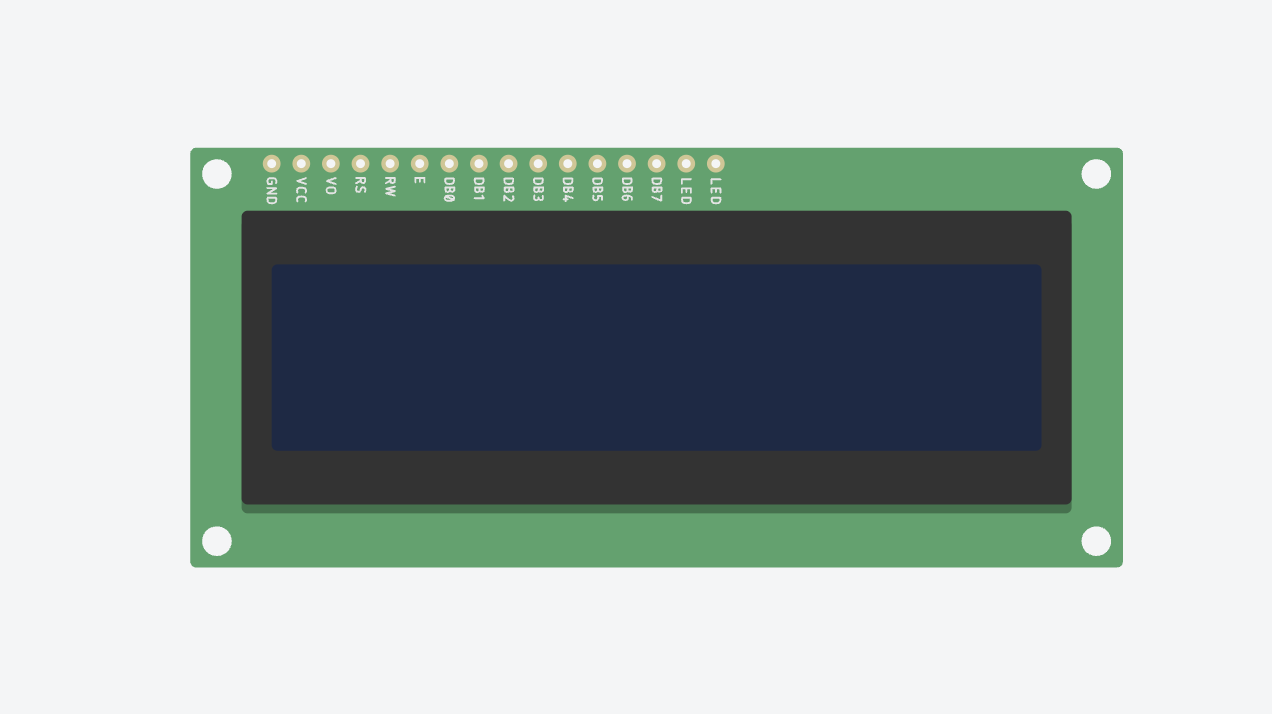
\includegraphics[width=0.5\linewidth]{figs/lcdpin.png}
\end{figure}
\subsection{Push Button Matrix}
\begin{itemize}
\item A push-button matrix is a method of reading multiple button inputs using a grid-like arrangement, reducing the number of required microcontroller pins. This is achieved by scanning rows and columns to detect button presses.
\item Here, we used it to efficiently interface multiple push buttons with the Arduino, allowing user input for calculator operations while conserving I/O pins.
\item Normally to implement 24 buttons we need 24 I/O pins, by using matrix connections we can reduce it to 10 pins 
\end{itemize}
\subsection*{Connections}
In my connections i have defined a 4x6 matrix for various functions 
\begin{figure}[H]
    \centering
    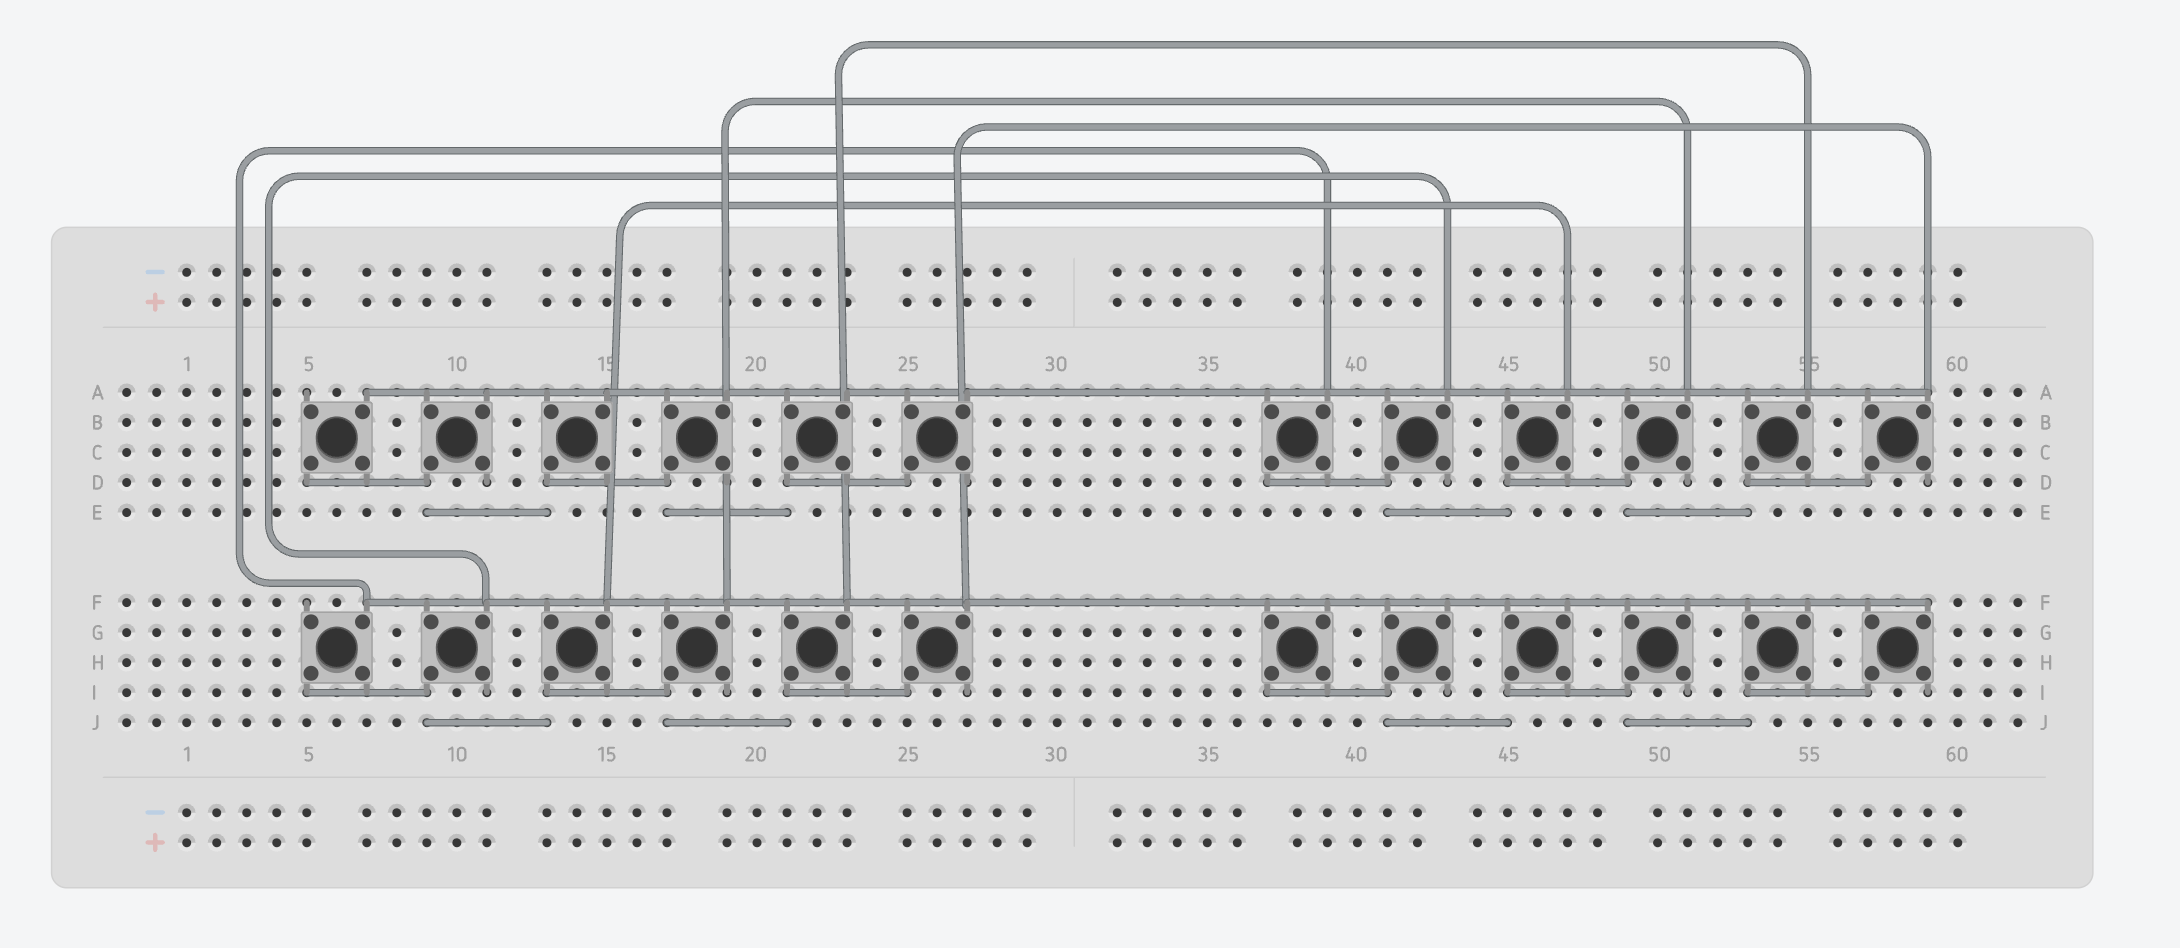
\includegraphics[width=0.7\linewidth]{figs/matrixpin.png}
\end{figure}
\begin{itemize}
    \item Connect one pin of the push button to all the rows and the final element of the rows to the arduino pins 
    \item Collect the pther pin of the push button to all the columns and the final element of each column to the arduino pins 
\end{itemize}
\subsection*{LCD Connections}
\begin{table}[H]
    \centering
    \begin{tabular}{|c|c|c|l|}
        \hline
        \textbf{LCD Pin} & \textbf{Name} & \textbf{Arduino Pin} & \textbf{Description} \\
        \hline
        1  & VSS   & GND  & Ground \\
        2  & VDD   & 5V   & Power Supply (5V) \\
        3  & V0    & Potentiometer(MiddlePin) & Contrast Adjustment \\
        4  & RS    & 7    & Register Select \\
        5  & RW    & GND  & Read/Write  \\
        6  & E     & 6    & Enable Pin \\
        7  & D0    & -    & Not used  \\
        8  & D1    & -    & Not used \\
        9  & D2    & -    & Not used \\
        10 & D3    & -    & Not used \\
        11 & D4    & 5    & Data Line 4 \\
        12 & D5    & 4    & Data Line 5 \\
        13 & D6    & 3    & Data Line 6 \\
        14 & D7    & 2    & Data Line 7 \\
        15 & LED+ & 5V  & LED Backlight Power \\
        16 & LED- & GND & LED Backlight Ground \\
        \hline
    \end{tabular}
\end{table}
Connect the other ends of the potentiometer to 5V and GND 
\subsection*{Keypad Connections}
\begin{table}[H]
    \centering
    \begin{tabular}{|c|c|}
        \hline
        \textbf{Keypad Pin} & \textbf{Arduino Pin}  \\
        \hline
        Row 1   & 9   \\
        Row 2   & 8   \\
        Row 3   & 7  \\
        Row 4   & 6  \\
        Column 1  & 5   \\
        Column 2  & 4   \\
        Column 3  & 3  \\
        Column 4  & 2  \\
        \hline
    \end{tabular}
\end{table}
\section{Working}
Power up the arduino and upload the following code 
\begin{lstlisting}[style=customC]
#include <avr/io.h>
#include <util/delay.h>
#include <stdlib.h>
#include <string.h>
#include <math.h>
#include <ctype.h>
#include <stdio.h>
#include <stdint.h>

// LCD Pin Definitions
// LCD Pin Definitions
#define LCD_RS_DDR      DDRD
#define LCD_RS_PORT     PORTD
#define LCD_RS_PIN      7

#define LCD_E_DDR       DDRD
#define LCD_E_PORT      PORTD
#define LCD_E_PIN       6

#define LCD_D4_DDR      DDRD
#define LCD_D4_PORT     PORTD
#define LCD_D4_PIN      5

#define LCD_D5_DDR      DDRD
#define LCD_D5_PORT     PORTD
#define LCD_D5_PIN      4

#define LCD_D6_DDR      DDRD
#define LCD_D6_PORT     PORTD
#define LCD_D6_PIN      3

#define LCD_D7_DDR      DDRD
#define LCD_D7_PORT     PORTD
#define LCD_D7_PIN      2

// Keypad Row Pin Definitions (Moved from Port A to Port C)
#define ROW1_DDR        DDRC
#define ROW1_PORT       PORTC
#define ROW1_PIN        PINC
#define ROW1_BIT        0

#define ROW2_DDR        DDRC
#define ROW2_PORT       PORTC
#define ROW2_PIN        PINC
#define ROW2_BIT        1

#define ROW3_DDR        DDRC
#define ROW3_PORT       PORTC
#define ROW3_PIN        PINC
#define ROW3_BIT        2

#define ROW4_DDR        DDRC
#define ROW4_PORT       PORTC
#define ROW4_PIN        PINC
#define ROW4_BIT        3

// Keypad Column Pin Definitions (Unchanged, using Port B)
#define COL1_DDR        DDRB
#define COL1_PORT       PORTB
#define COL1_PIN        PINB
#define COL1_BIT        0

#define COL2_DDR        DDRB
#define COL2_PORT       PORTB
#define COL2_PIN        PINB
#define COL2_BIT        1

#define COL3_DDR        DDRB
#define COL3_PORT       PORTB
#define COL3_PIN        PINB
#define COL3_BIT        2

#define COL4_DDR        DDRB
#define COL4_PORT       PORTB
#define COL4_PIN        PINB
#define COL4_BIT        3

#define COL5_DDR        DDRB
#define COL5_PORT       PORTB
#define COL5_PIN        PINB
#define COL5_BIT        4

#define COL6_DDR        DDRB
#define COL6_PORT       PORTB
#define COL6_PIN        PINB
#define COL6_BIT        5


// Keypad dimensions
#define ROW_NUM    4
#define COLUMN_NUM 6

// Character mapping for keypad
char keys[ROW_NUM][COLUMN_NUM] = {
  {'1', '2', '3', '+' , '-', '*'},
  {'4', '5', '6', '/' , 'C', '='},
  {'7', '8', '9', 'Q' , 'M', 'D'}, 
  {'0', 'e', 's' , 'c' , 't', 'S'}
};

// Arrays for row and column bits
uint8_t row_bits[ROW_NUM] = {ROW1_BIT, ROW2_BIT, ROW3_BIT, ROW4_BIT};
uint8_t col_bits[COLUMN_NUM] = {COL1_BIT, COL2_BIT, COL3_BIT, COL4_BIT, COL5_BIT, COL6_BIT};

// Variables to store input and shift state
char expression[32] = "";
uint8_t expr_length = 0;
uint8_t lastCharOperator = 0;  // Prevents consecutive operators
uint8_t shiftActive = 0;       // Flag for shift function (Inverse trig functions)

// Matrix A and B inputs
float A[2][2], B[2][2], C[2][2];

// LCD Commands
#define LCD_CLEAR           0x01
#define LCD_HOME            0x02
#define LCD_ENTRY_MODE      0x06
#define LCD_DISPLAY_ON      0x0C
#define LCD_FUNCTION_SET    0x28
#define LCD_SET_DDRAM       0x80

char buffer[32]; // Buffer for string conversion

// Function to determine operator precedence
int precedence(char op) {
  if (op == '+' || op == '-') return 1;
  if (op == '*' || op == '/') return 2;
  return 0;
}

// Function to apply an operation to two numbers
float applyOperation(float a, float b, char op) {
  switch (op) {
    case '+': return a + b;
    case '-': return a - b;
    case '*': return a * b;
    case '/': return (b != 0) ? a / b : 0;
  }
  return 0;
}

// LCD Functions
void lcd_send_nibble(uint8_t nibble) {
    // Set data pins according to nibble (higher 4 bits)
    if (nibble & 0x01) LCD_D4_PORT |= (1 << LCD_D4_PIN); else LCD_D4_PORT &= ~(1 << LCD_D4_PIN);
    if (nibble & 0x02) LCD_D5_PORT |= (1 << LCD_D5_PIN); else LCD_D5_PORT &= ~(1 << LCD_D5_PIN);
    if (nibble & 0x04) LCD_D6_PORT |= (1 << LCD_D6_PIN); else LCD_D6_PORT &= ~(1 << LCD_D6_PIN);
    if (nibble & 0x08) LCD_D7_PORT |= (1 << LCD_D7_PIN); else LCD_D7_PORT &= ~(1 << LCD_D7_PIN);
    
    // Pulse E pin
    LCD_E_PORT |= (1 << LCD_E_PIN);
    _delay_us(1);
    LCD_E_PORT &= ~(1 << LCD_E_PIN);
    _delay_us(100);
}

void lcd_command(uint8_t cmd) {
    LCD_RS_PORT &= ~(1 << LCD_RS_PIN);   // RS = 0 for command
    
    // Send high nibble
    lcd_send_nibble(cmd >> 4);
    
    // Send low nibble
    lcd_send_nibble(cmd & 0x0F);
    
    if (cmd == LCD_CLEAR || cmd == LCD_HOME)
        _delay_ms(2);  // These commands take longer
    else
        _delay_us(50);
}

void lcd_data(uint8_t data) {
    LCD_RS_PORT |= (1 << LCD_RS_PIN);    // RS = 1 for data
    
    // Send high nibble
    lcd_send_nibble(data >> 4);
    
    // Send low nibble
    lcd_send_nibble(data & 0x0F);
    
    _delay_us(50);
}

void lcd_init(void) {
    // Set data pins as output
    LCD_RS_DDR |= (1 << LCD_RS_PIN);
    LCD_E_DDR |= (1 << LCD_E_PIN);
    LCD_D4_DDR |= (1 << LCD_D4_PIN);
    LCD_D5_DDR |= (1 << LCD_D5_PIN);
    LCD_D6_DDR |= (1 << LCD_D6_PIN);
    LCD_D7_DDR |= (1 << LCD_D7_PIN);
    
    _delay_ms(50);    // Wait for LCD to power up
    
    // Initialize in 4-bit mode
    LCD_RS_PORT &= ~(1 << LCD_RS_PIN);   // RS = 0 for command
    
    // Send 0x03 three times (initialization sequence)
    lcd_send_nibble(0x03);
    _delay_ms(5);
    
    lcd_send_nibble(0x03);
    _delay_ms(5);
    
    lcd_send_nibble(0x03);
    _delay_ms(5);
    
    // Now set to 4-bit mode
    lcd_send_nibble(0x02);
    _delay_ms(5);
    
    // Now officially in 4-bit mode, send commands
    lcd_command(LCD_FUNCTION_SET);   // 4-bit, 2 lines, 5x8 font
    lcd_command(LCD_DISPLAY_ON);     // Display on, cursor off, no blink
    lcd_command(LCD_CLEAR);          // Clear display
    lcd_command(LCD_ENTRY_MODE);     // Increment cursor, no display shift
    
    _delay_ms(2);
}

void lcd_string(const char *str) {
    while (*str) {
        lcd_data(*str++);
    }
}

void lcd_set_cursor(uint8_t row, uint8_t col) {
    uint8_t address;
    
    if (row == 0)
        address = 0x00 + col;
    else if (row == 1)
        address = 0x40 + col;
    else if (row == 2)
        address = 0x14 + col;
    else
        address = 0x54 + col;
        
    lcd_command(LCD_SET_DDRAM | address);
}

void lcd_clear(void) {
    lcd_command(LCD_CLEAR);
    _delay_ms(2);
}

// Keypad Functions
void keypad_init(void) {
    // Set row pins as input with pull-ups
    ROW1_DDR &= ~(1 << ROW1_BIT);
    ROW2_DDR &= ~(1 << ROW2_BIT);
    ROW3_DDR &= ~(1 << ROW3_BIT);
    ROW4_DDR &= ~(1 << ROW4_BIT);
    
    ROW1_PORT |= (1 << ROW1_BIT);
    ROW2_PORT |= (1 << ROW2_BIT);
    ROW3_PORT |= (1 << ROW3_BIT);
    ROW4_PORT |= (1 << ROW4_BIT);
    
    // Set column pins as output and set high
    COL1_DDR |= (1 << COL1_BIT);
    COL2_DDR |= (1 << COL2_BIT);
    COL3_DDR |= (1 << COL3_BIT);
    COL4_DDR |= (1 << COL4_BIT);
    COL5_DDR |= (1 << COL5_BIT);
    COL6_DDR |= (1 << COL6_BIT);
    
    COL1_PORT |= (1 << COL1_BIT);
    COL2_PORT |= (1 << COL2_BIT);
    COL3_PORT |= (1 << COL3_BIT);
    COL4_PORT |= (1 << COL4_BIT);
    COL5_PORT |= (1 << COL5_BIT);
    COL6_PORT |= (1 << COL6_BIT);
}

char get_key(void) {
    uint8_t r, c;
    
    // Check for keypress by scanning the keypad
    for (c = 0; c < COLUMN_NUM; c++) {
        // Set current column to low
        switch(c) {
            case 0: COL1_PORT &= ~(1 << COL1_BIT); break;
            case 1: COL2_PORT &= ~(1 << COL2_BIT); break;
            case 2: COL3_PORT &= ~(1 << COL3_BIT); break;
            case 3: COL4_PORT &= ~(1 << COL4_BIT); break;
            case 4: COL5_PORT &= ~(1 << COL5_BIT); break;
            case 5: COL6_PORT &= ~(1 << COL6_BIT); break;
        }
        
        _delay_us(10); // Small delay for stabilization
        
        // Check each row
        for (r = 0; r < ROW_NUM; r++) {
            uint8_t row_val = 0;
            
            switch(r) {
                case 0: row_val = !(ROW1_PIN & (1 << ROW1_BIT)); break;
                case 1: row_val = !(ROW2_PIN & (1 << ROW2_BIT)); break;
                case 2: row_val = !(ROW3_PIN & (1 << ROW3_BIT)); break;
                case 3: row_val = !(ROW4_PIN & (1 << ROW4_BIT)); break;
            }
            
            if (row_val) {  // Key is pressed
                // Set column back to high
                switch(c) {
                    case 0: COL1_PORT |= (1 << COL1_BIT); break;
                    case 1: COL2_PORT |= (1 << COL2_BIT); break;
                    case 2: COL3_PORT |= (1 << COL3_BIT); break;
                    case 3: COL4_PORT |= (1 << COL4_BIT); break;
                    case 4: COL5_PORT |= (1 << COL5_BIT); break;
                    case 5: COL6_PORT |= (1 << COL6_BIT); break;
                }
                
                _delay_ms(20); // Debounce delay
                return keys[r][c];
            }
        }
        
        // Set column back to high
        switch(c) {
            case 0: COL1_PORT |= (1 << COL1_BIT); break;
            case 1: COL2_PORT |= (1 << COL2_BIT); break;
            case 2: COL3_PORT |= (1 << COL3_BIT); break;
            case 3: COL4_PORT |= (1 << COL4_BIT); break;
            case 4: COL5_PORT |= (1 << COL5_BIT); break;
            case 5: COL6_PORT |= (1 << COL6_BIT); break;
        }
    }
    
    return 0;  // No key pressed
}

// Function to evaluate an expression using BODMAS
float evaluateExpression(char *expr) {
  float values[16]; // Stack for numbers
  char ops[16];     // Stack for operators
  int valTop = -1, opTop = -1;
  int i = 0;

  while (expr[i] != '\0') {
    if (isdigit(expr[i]) || expr[i] == '.') {
      char num[16] = "";
      int j = 0;
      while (expr[i] != '\0' && (isdigit(expr[i]) || expr[i] == '.')) {
        num[j++] = expr[i++];
      }
      num[j] = '\0';
      values[++valTop] = atof(num);
      i--;  // Adjust index
    } else {
      while (opTop >= 0 && precedence(ops[opTop]) >= precedence(expr[i])) {
        float b = values[valTop--];
        float a = values[valTop--];
        char op = ops[opTop--];
        values[++valTop] = applyOperation(a, b, op);
      }
      ops[++opTop] = expr[i];
    }
    i++;
  }

  while (opTop >= 0) {
    float b = values[valTop--];
    float a = values[valTop--];
    char op = ops[opTop--];
    values[++valTop] = applyOperation(a, b, op);
  }

  return values[0];  // Final result
}

// Function to handle trigonometric calculations (sin, cos, tan)
float trigFunction(char func, float angle) {
  // Convert angle from degrees to radians before performing trig operations
  float radians = angle * (M_PI / 180.0);
  
  if (shiftActive) {  // Inverse trigonometric functions (asin, acos, atan)
    switch (func) {
      case 's':  // Inverse sin (asin)
        if (angle >= -1 && angle <= 1) {
          return asin(angle) * (180.0 / M_PI);  // Convert result back to degrees
        } else {
          lcd_clear();
          lcd_string("asin: Invalid input");
          _delay_ms(2000);
          return 0;  // Error message if out of range
        }
      case 'c':  // Inverse cos (acos)
        if (angle >= -1 && angle <= 1) {
          return acos(angle) * (180.0 / M_PI);
        } else {
          lcd_clear();
          lcd_string("acos: Invalid input");
          _delay_ms(2000);
          return 0;  // Error message if out of range
        }
      case 't':  // Inverse tan (atan)
        return atan(angle) * (180.0 / M_PI);  // atan is valid for any real number
    }
  } else {  // Regular sin, cos, tan functions
    switch (func) {
      case 's':  // sin
        return sin(radians);
      case 'c':  // cos
        return cos(radians);
      case 't':  // tan
        return tan(radians);
    }
  }
  return 0;
}

// Function to handle the 'e^x' functionality
void handleExponent(void) {
  lcd_clear();
  lcd_string("Enter x:");
  char numStr[16] = "";
  int numIdx = 0;
  
  while (1) {
    char key = get_key();
    if (key) {
      if (isdigit(key) || key == '.') {
        numStr[numIdx++] = key;
        numStr[numIdx] = '\0';
        lcd_data(key);
      } 
      else if (key == '=') {
        float exponent = atof(numStr);
        float result = exp(exponent);  // Calculate e^x
        lcd_clear();
        lcd_string("e^x = ");
        
        // Convert float to string
        dtostrf(result, 6, 2, buffer);
        lcd_string(buffer);
        
        _delay_ms(2000);
        lcd_clear();
        break;
      }
    }
    _delay_ms(100); // Debounce
  }
}

// Function to input matrix A and B
float getMatrixElement(char matrixName, int row, int col) {
    lcd_clear();
    lcd_string("Enter ");
    lcd_data(matrixName);  
    lcd_string("[");
    lcd_data('0' + row);  
    lcd_string("][");
    lcd_data('0' + col);  
    lcd_string("]: ");

    char inputStr[16] = "";  
    int inputIdx = 0;

    while (1) {
        char key = get_key();  

        if (key) {
            if ((key >= '0' && key <= '9') || key == '.' || key == '-') {  // Allow digits, decimal, and negative sign
                if (inputIdx < 15) {  // Prevent buffer overflow
                    inputStr[inputIdx++] = key;
                    inputStr[inputIdx] = '\0';
                    lcd_data(key);  // Display typed key
                }
            } 
            else if (key == '=') {  // Confirm input
                break;
            }
        }
        _delay_ms(100);  // Debounce delay
    }

    return atof(inputStr);  // Convert input string to float
}

void inputMatrices(void) {
    lcd_clear();
    lcd_string("Enter A:");

    A[0][0] = getMatrixElement('A', 1, 1);  // A11
    _delay_ms(500);  

    A[0][1] = getMatrixElement('A', 1, 2);  // A12
    _delay_ms(500);  

    A[1][0] = getMatrixElement('A', 2, 1);  // A21
    _delay_ms(500);  

    A[1][1] = getMatrixElement('A', 2, 2);  // A22
    _delay_ms(500);  

    lcd_clear();
    lcd_string("Enter B:");

    B[0][0] = getMatrixElement('B', 1, 1);  // B11
    _delay_ms(500);  

    B[0][1] = getMatrixElement('B', 1, 2);  // B12
    _delay_ms(500);  

    B[1][0] = getMatrixElement('B', 2, 1);  // B21
    _delay_ms(500);  

    B[1][1] = getMatrixElement('B', 2, 2);  // B22
    _delay_ms(500);  
}

// Function to perform matrix addition

void matrixAddition(void) {
    for (int i = 0; i < 2; i++) {
        for (int j = 0; j < 2; j++) {
            C[i][j] = A[i][j] + B[i][j];  // Correct formula for addition
        }
    }
}

// Function to perform matrix multiplication
void matrixMultiplication(void) {
    float tempC[2][2] = {0}; // Temporary matrix to avoid overwriting errors

    for (int i = 0; i < 2; i++) {
        for (int j = 0; j < 2; j++) {
            tempC[i][j] = (A[i][0] * B[0][j]) + (A[i][1] * B[1][j]);  // Correct multiplication formula
        }
    }

    // Copy result to C
    for (int i = 0; i < 2; i++) {
        for (int j = 0; j < 2; j++) {
            C[i][j] = tempC[i][j];
        }
    }
}



// Function to handle shift toggle
void toggleShift(void) {
  shiftActive = !shiftActive;
  lcd_clear();
  if (shiftActive) {
    lcd_string("Inverse Mode");
  } else {
    lcd_string("Calculator Ready");
    _delay_ms(2000);
  }
  _delay_ms(1000);  // Show shift status for 1 second
  lcd_clear();
}

// Function to get input for angle
float getInput(void) {
  lcd_clear();
  lcd_string("Enter Angle: ");
  char angleStr[16] = "";
  int angleIdx = 0;
  
  while (1) {
    char key = get_key();
    if (key) {
      if (isdigit(key) || key == '.') {
        angleStr[angleIdx++] = key;
        angleStr[angleIdx] = '\0';
        lcd_data(key);
      } else if (key == '=') {
        break;
      }
    }
    _delay_ms(100); // Debounce
  }
  
  return atof(angleStr);  // Convert input to float and return
}

// Function to get quadratic input
char buffer1[16], buffer2[16];

float getQuadraticInput(const char* prompt) {
    lcd_clear();
    lcd_string(prompt);
    char inputStr[16] = ""; // Buffer for input
    int inputIdx = 0;
    
    while (1) {
        char key = get_key(); // Read keypress
        if (key) {
            if (isdigit(key) || key == '.' || key == '-') {  // Support negative numbers
                if (inputIdx < 15) { // Prevent buffer overflow
                    inputStr[inputIdx++] = key;
                    inputStr[inputIdx] = '\0';
                    lcd_data(key);
                }
            } else if (key == '=') {  // Enter key (confirmation)
                break;
            }
        }
        _delay_ms(100); // Debounce
    }
    
    return atof(inputStr); // Convert input string to float
}


// Function to get differentiation input
void getDifferentiationInput(float coeffs[], float powers[], int *termCount) {
  lcd_clear();
  lcd_string("Enter f(x):");
  _delay_ms(1000);
  
  char numStr[16] = "";
  int numIdx = 0;
  *termCount = 0;
  uint8_t expectingPower = 0;
  uint8_t expectingOperator = 0;

  while (1) {
    char key = get_key();
    if (key) {
      if (isdigit(key) || key == '.') {
        numStr[numIdx++] = key;
        numStr[numIdx] = '\0';
        lcd_data(key);
        expectingOperator = 0;
      }
      else if (key == 'x' || key == '*') {  // Treat '*' as 'x' (multiplication)
        if (numIdx > 0) {  // If there is a coefficient before 'x'
          coeffs[*termCount] = atof(numStr);
        } else {
          coeffs[*termCount] = 1;  // Default coefficient is 1 if not specified
        }
        numIdx = 0;
        numStr[0] = '\0';
        lcd_data('x');  // Show 'x' for multiplication
        expectingPower = 1;  // Expecting the power after 'x'
      }
      else if (key == '+' || key == '-') {  // Handle + and - for next term
        if (numIdx > 0 && expectingPower) {
          powers[*termCount] = atof(numStr);
          numIdx = 0;
          numStr[0] = '\0';
        } else if (numIdx > 0) {
          coeffs[*termCount] = atof(numStr);
          powers[*termCount] = 0;  // If no 'x', power is 0 (constant term)
          numIdx = 0;
          numStr[0] = '\0';
        }
        
        if (expectingPower && numIdx == 0) {
          powers[*termCount] = 1;  // Default power is 1 if not specified after 'x'
        }
        
        (*termCount)++;
        lcd_data(key);
        expectingPower = 0;
        expectingOperator = 1;
      }
      else if (key == '=') {  // Finish input
        if (numIdx > 0) {
          if (expectingPower) {
            powers[*termCount] = atof(numStr);
          } else {
            coeffs[*termCount] = atof(numStr);
            powers[*termCount] = 0;  // Constant term
          }
        }
        
        if (expectingPower && numIdx == 0) {
          powers[*termCount] = 1;  // Default power is 1 if not specified after 'x'
        }
        
        (*termCount)++;
        break;
      }
    }
    _delay_ms(100); // Debounce
  }
}

// Differentiation function
void differentiateFunction(void) {
  float coeffs[10] = {0}, powers[10] = {0};
  int termCount = 0;
  
  getDifferentiationInput(coeffs, powers, &termCount);

  lcd_clear();
  lcd_string("f(x)=");
  uint8_t firstTerm = 1;
  for (int i = 0; i < termCount; i++) {
    if (coeffs[i] != 0) {  // Only print non-zero coefficients
      if (!firstTerm && coeffs[i] > 0) lcd_data('+');
      
      // Convert coefficient to string
      dtostrf(coeffs[i], 3, 1, buffer);
      lcd_string(buffer);
      
      if (powers[i] != 0) {  // If not a constant term
        lcd_data('x');
        
        if (powers[i] != 1) {  // Only show power if not 1
          lcd_data('^');
          
          // Convert power to string
          dtostrf(powers[i], 2, 0, buffer);
          lcd_string(buffer);
        }
      }
      
      firstTerm = 0;
    }
  }

  lcd_set_cursor(0, 1);
  lcd_string("f'(x)=");
  firstTerm = 1;
  for (int i = 0; i < termCount; i++) {
    if (powers[i] != 0 && coeffs[i] != 0) {
      float derivativeCoeff = coeffs[i] * powers[i];
      float derivativePower = powers[i] - 1;
      
      if (!firstTerm && derivativeCoeff > 0) lcd_data('+');
      
      // Convert derivative coefficient to string
      dtostrf(derivativeCoeff, 3, 1, buffer);
      lcd_string(buffer);
      
      if (derivativePower != 0) {  // Only show x if power is not 0 after differentiation
        lcd_data('x');
        
        if (derivativePower != 1) {  // Only show power if not 1
          lcd_data('^');
          
          // Convert derivative power to string
          dtostrf(derivativePower, 2, 0, buffer);
          lcd_string(buffer);
        }
      }
      
      firstTerm = 0;
    }
  }

  _delay_ms(5000);
  lcd_clear();
}

// Function to solve quadratic equations
void inputQuadraticCoefficients(void) {
    float a2, a1, a0;

    // Prompt and get inputs
    a2 = getQuadraticInput("Enter a2: ");  
    _delay_ms(500); // Short delay before next prompt
    
    a1 = getQuadraticInput("Enter a1: ");
    _delay_ms(500);
    
    a0 = getQuadraticInput("Enter a0: ");  
    _delay_ms(500);

    // Check if it's a valid quadratic equation
    if (a2 == 0) {
        lcd_clear();
        lcd_string("Not a quadratic");
        _delay_ms(2000);
        return;
    }

    // Calculate discriminant
    float delta = a1 * a1 - 4 * a0 * a2;
    lcd_clear();

    if (delta < 0) {
        lcd_string("No real roots");
    } else {
        float root1 = (-a1 + sqrt(delta)) / (2 * a2);
        float root2 = (-a1 - sqrt(delta)) / (2 * a2);
        
        // Convert roots to strings
        dtostrf(root1, 6, 2, buffer1);
        dtostrf(root2, 6, 2, buffer2);
        
        // **FIX: Clear LCD again before printing**
        lcd_clear();
        _delay_ms(50);  // Small delay for LCD stability

        // **Ensure correct LCD positioning**
        lcd_set_cursor(0, 0);
        lcd_string("Root1: ");
        lcd_string(buffer1);

        lcd_set_cursor(0, 1);
        lcd_string("Root2: ");
        lcd_string(buffer2);
    }
    _delay_ms(3000);
}
// Function to display the result matrix C
void displayMatrix(void) {
    lcd_clear();
    
    char buffer[10];

    // Display first row of result matrix C (C11 C12)
    lcd_set_cursor(0, 0);  // First row
    dtostrf(C[0][0], 6, 2, buffer);
    lcd_string(buffer);
    lcd_string(" ");  
    dtostrf(C[0][1], 6, 2, buffer);
    lcd_string(buffer);

    // **FORCE CURSOR TO NEXT LINE**
    _delay_ms(3000); // Small delay to allow LCD to process
    lcd_set_cursor(0, 1);  // Move to second row

    // Display second row of result matrix C (C21 C22)
    dtostrf(C[1][0], 6, 2, buffer);
    lcd_string(buffer);
    lcd_string(" ");  
    dtostrf(C[1][1], 6, 2, buffer);
    lcd_string(buffer);
}


void matrixOperations(void) {
    lcd_clear();
    lcd_string("Matrix Ops");
    _delay_ms(500);

    // Input Matrices
    inputMatrices();

    // Ask user for operation choice
    lcd_clear();
    lcd_string("3: A+B  4: A*B");

    char key;
    while (1) {
        key = get_key();
        if (key == '3') {
            matrixAddition();
            displayMatrix();
            break;
        } else if (key == '4') {
            matrixMultiplication();
            displayMatrix();
            break;
        }
    }
}
int main(void) {
  // Initialize LCD and Keypad
  lcd_init();
  keypad_init();
  
  // Display welcome message
  lcd_string("Sci Calculator");
  _delay_ms(2000);  
  lcd_clear();
  
  while (1) {
    char key = get_key();
    
    if (key) {
      if (key == 'C') {  // C button clears the screen
        lcd_clear();  // Clears the LCD
        expr_length = 0;
        expression[0] = '\0';
        lastCharOperator = 0;
      }
      else if (key == 'S') {  // Shift button toggles inverse mode
        toggleShift();
      }
      else if (key == 'e') {  // Exponential function (e^x)
        handleExponent();
      }
      else if (key == 'Q') {  // Quadratic equation solver
        inputQuadraticCoefficients();
      }
      else if (key == 'D') {  // Differentiation
        differentiateFunction();
      }
      else if (key == 'M') {  // Matrix operations
        lcd_clear();
        matrixOperations();
      
      }
      else if (key == 's' || key == 'c' || key == 't') {  // Trigonometric functions
        float angle = getInput();
        float result = trigFunction(key, angle);
        
        lcd_clear();
        if (shiftActive) {
          lcd_data('a');  // Display 'a' for inverse trig functions
        }
        
        if (key == 's') lcd_string("sin(");
        else if (key == 'c') lcd_string("cos(");
        else if (key == 't') lcd_string("tan(");
        
        // Convert angle to string
        dtostrf(angle, 4, 1, buffer);
        lcd_string(buffer);
        lcd_string(") = ");
        
        // Convert result to string
        dtostrf(result, 6, 4, buffer);
        lcd_string(buffer);
        
        _delay_ms(3000);
        lcd_clear();
      }
      else if (key == '=') {  // Evaluate expression
        if (expr_length > 0) {
          float result = evaluateExpression(expression);
          lcd_clear();
          lcd_string("= ");
          
          // Convert result to string
          dtostrf(result, 10, 4, buffer);
          lcd_string(buffer);
          
          _delay_ms(3000);
          lcd_clear();
          
          // Reset expression for a new calculation
          expr_length = 0;
          expression[0] = '\0';
          lastCharOperator = 0;
        }
      }
      else {  // Regular input (digits, operators)
        if (isdigit(key) || key == '.') {
          if (expr_length < 31) {  // Check for buffer overflow
            expression[expr_length++] = key;
            expression[expr_length] = '\0';
            lcd_data(key);
            lastCharOperator = 0;
          }
        }
        else if (key == '+' || key == '-' || key == '*' || key == '/') {
          if (expr_length > 0 && !lastCharOperator) {  // Prevent consecutive operators
            if (expr_length < 31) {
              expression[expr_length++] = key;
              expression[expr_length] = '\0';
              lcd_data(key);
              lastCharOperator = 1;
            }
          }
          else if (key == '-' && expr_length == 0) {  // Allow negative at start
            expression[expr_length++] = key;
            expression[expr_length] = '\0';
            lcd_data(key);
            lastCharOperator = 0;  // Special case for negative at start
          }
        }
      }
    }
    _delay_ms(100);  // Debounce delay
  }
  
  return 0;  // Never reached
}
\end{lstlisting}
The keypad matrix is given below
\begin{figure}[H]
    \centering
    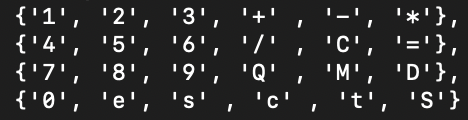
\includegraphics[width=0.5\linewidth]{figs/keypadlayout.png}
\end{figure}
Push Button Functions 
\begin{itemize}
    \item \textbf{Numeric Keys (0-9)}: Used to enter numerical values.
    \item \textbf{Arithmetic Operators ($\div, \times, -, +$)}: Perform basic arithmetic operations.
    \item \textbf{Exponential : $e^x$}: Calculates the value of e raised to the power x 
    \item \textbf{Shift : S}: The shift button is used to toggle between trigonometric functions and inverse trigonometric functions of sin cos tan 
    \item \textbf{Equal (=)}: Evaluates the entered expression.
    \item \textbf{Differentiate (D)}: Computes the derivative of an entered function.
    \item \textbf{Quadratic Solver : Q}: Quadratic equation solver it takes values a2 a1 a0 from the user and computes the roots of the quadratic equation 
    \begin{itemize}
        \item If a2 = 0 , it shows not a quadratic 
        \item If $\Delta < 0 $, it shows no real roots 
        \item It shows Root 1 in line 1 and Root 2 in line 2 
    \end{itemize}
    \item \textbf{Differentiator : D}: It computes the derivative of a function f(x) taking input f(x) from the user 
    \begin{itemize}
        \item It also identifies operators + - * /
        \item the number after x is consider as its power until any operator is recognised 
    \end{itemize}
    \item \textbf{Matrix Operator : M}: It takes two 2x2 matrices A and B and gives outputs addition and multiplication 
    \begin{itemize}
        \item It takes A and B matrices as inputs 
        \item Then it asks the user 3:A+B 4:AXB, after choosing an option 
        \item It displays the output matrix on the lcd 
    \end{itemize}
      
    
\end{itemize}
\section{Results}
\begin{itemize}
    \item[1.] Open terminal and go to your working directory 
\begin{tcolorbox}[colback=gray!15, colframe=black, sharp corners, boxrule=0.5pt, left=2mm, right=2mm, top=1mm, bottom=1mm]
\texttt{cd /sdcard/cprog/src}
\end{tcolorbox}
\item[2.] Write you code calculator.c inside src 
\begin{tcolorbox}[colback=gray!15, colframe=black, sharp corners, boxrule=0.5pt, left=2mm, right=2mm, top=1mm, bottom=1mm]
\texttt{nvim calculator.c}
\end{tcolorbox}
\item[3.] Execute the avr-gcc code using the below command, which creates .hex file 
\begin{tcolorbox}[colback=gray!15, colframe=black, sharp corners, boxrule=0.5pt, left=2mm, right=2mm, top=1mm, bottom=1mm]
\texttt{avr-gcc -mmcu=atmega328p -Os -o calculator.elf calculator.c \&\& avr-objcopy -O ihex calculator.elf calculator.hex}
\end{tcolorbox}
\item[4.]Copy that .hex file into ArduinoDroid directory 
\begin{tcolorbox}[colback=gray!15, colframe=black, sharp corners, boxrule=0.5pt, left=2mm, right=2mm, top=1mm, bottom=1mm]
\texttt{cp calculator.hex /sdcard/ArduinoDroid/precompiled}
\end{tcolorbox}
\item[5.] Upload the precompiled code to the arduino using USB 
\end{itemize}
\begin{figure}[H]
    \centering
    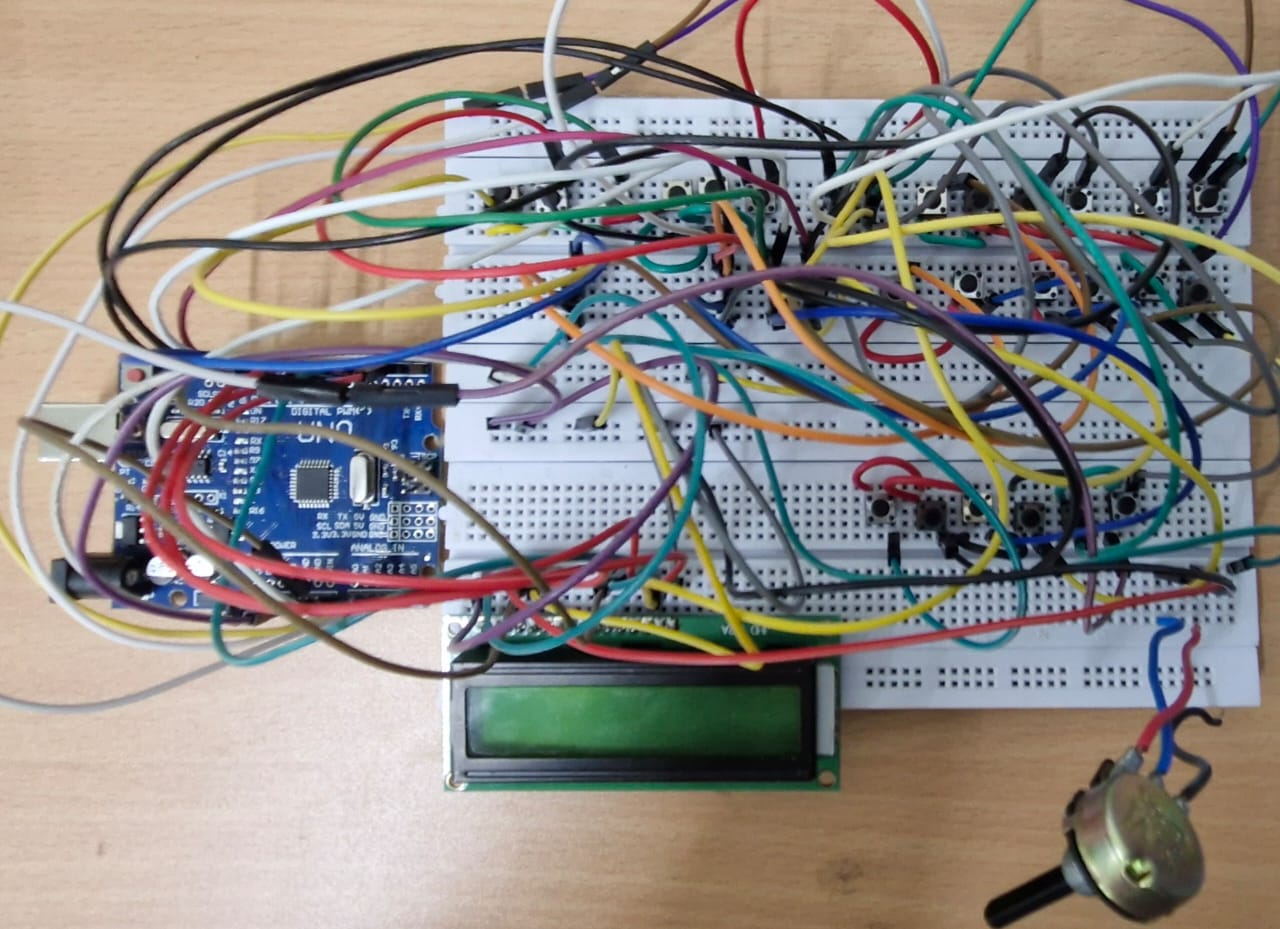
\includegraphics[width=0.7\linewidth]{figs/calcbread.jpeg}
\end{figure}

\end{document}